\begin{figure}[t]
    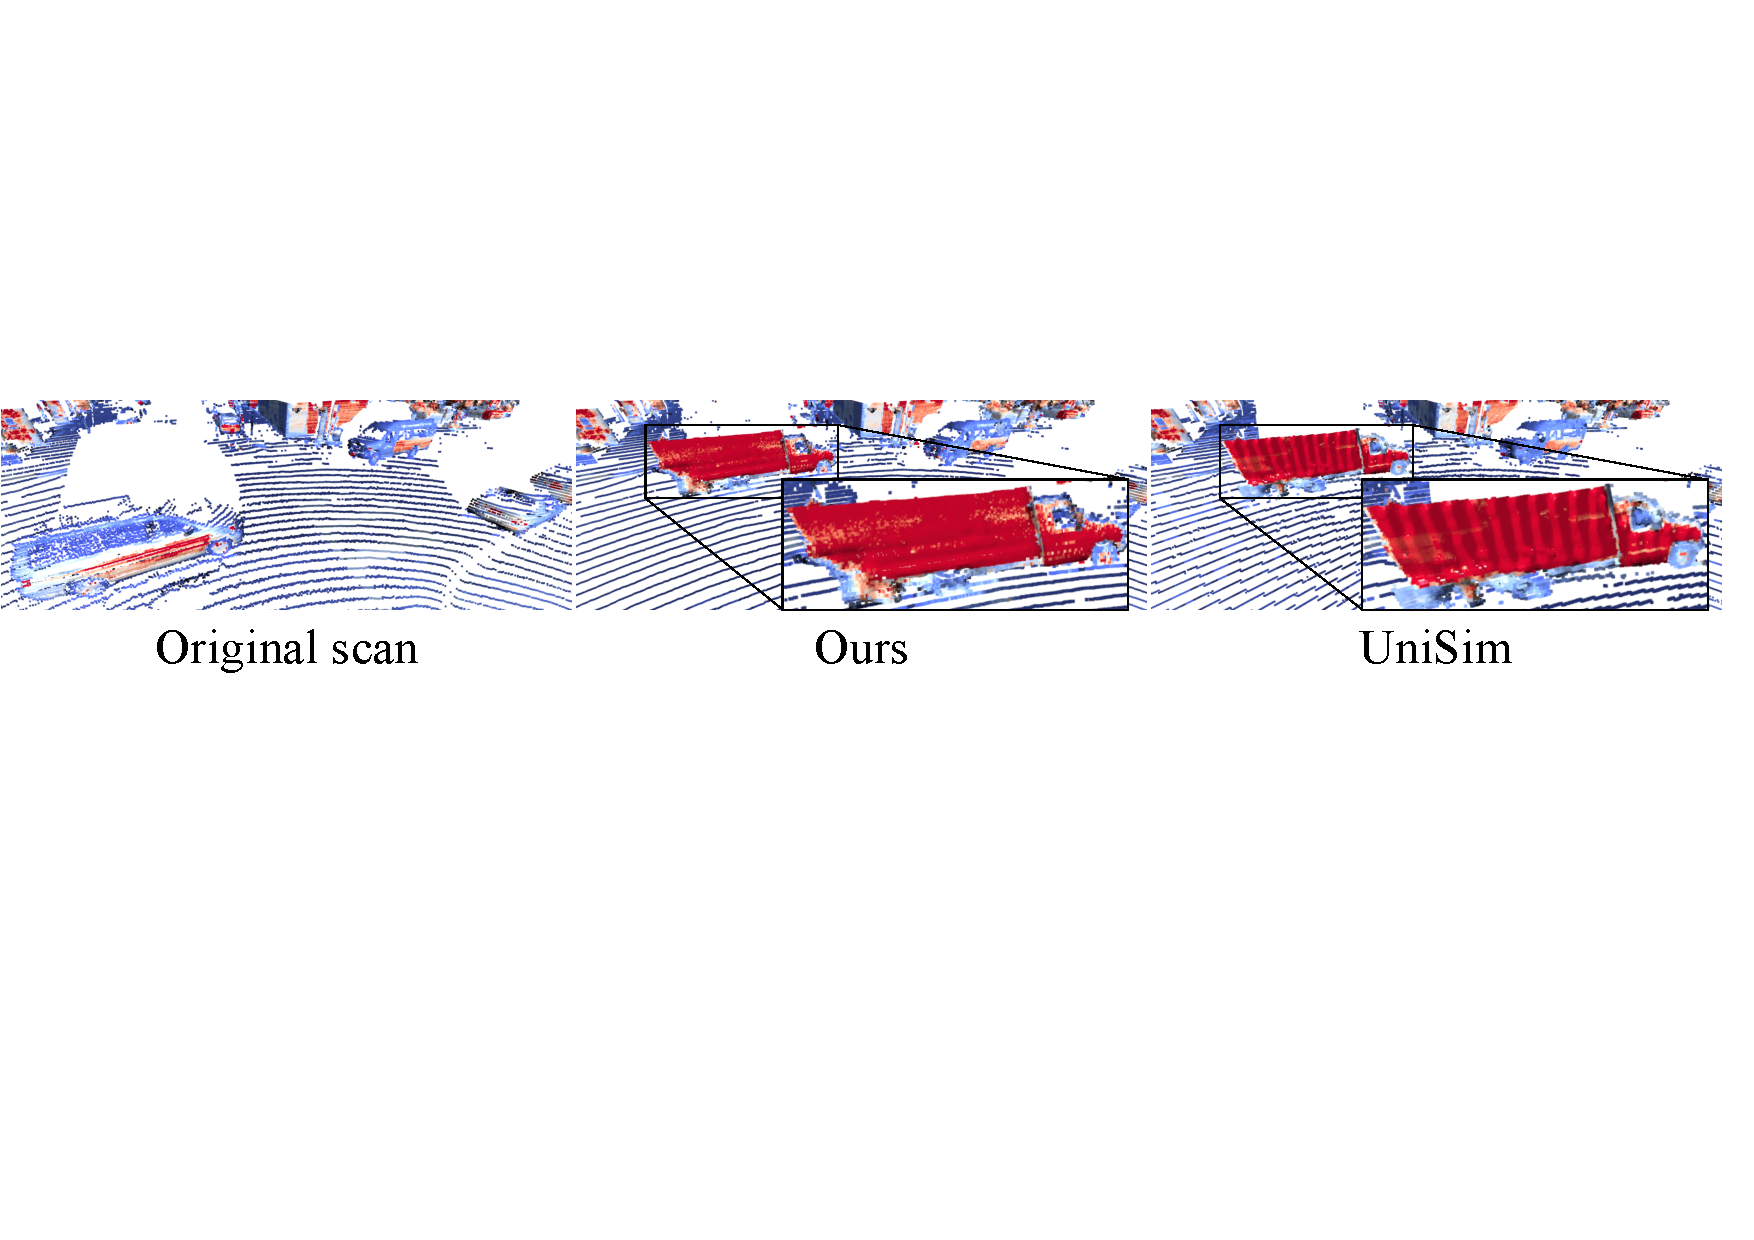
\includegraphics[width=1.0\linewidth]{Figures/vehicle_insertion.pdf}
    
    % \caption{
    % Object removal and insertion comparison between ours and UniSim~\cite{yang2023unisim}. The vehicle from the GT is removed and the inserted vehicle is zoomed in for each method. The images are color coded by the intensity values (0 \bwrDyNFL~0.25)
    % }
    \caption{
    Qualitative results of object removal and insertion. \dynfl seamlessly inserts the neural asset (truck) into a new scene attributed to our superior compositional rendering scheme. In contrast, UniSim~\cite{yang2023unisim} struggles to accurately model geometry.
    }
    \label{fig:vehicle_insertion}
\end{figure}